\documentclass{article}
\usepackage[utf8]{inputenc}

\usepackage[letterpaper, margin=1in]{geometry}
\usepackage{amsmath}
\usepackage{enumitem}
\usepackage{caption}
\usepackage{subcaption}
\usepackage{graphicx}
\graphicspath{ {figures/} }

\title{Analytical model of pedestrianized and transit priority zones in a rectilinear grid city}
\author{Nicholas Fournier}
\date{February 2020}

\begin{document}


\maketitle

\section{Concept}
Consider an idealized city of dimension $R$ with a rectilinear street network with spacing $d$, as shown in Figure~\ref{fig:gridcity}. Demand can be defined by two types of trip patterns, baseline uniform travel demand across the city and monocentric trips to and from the city center. The cumulative effect is increased congestion in the city center. To make the city center more attractive, ``livable'', and walkable, a square zone of size $\gamma$ in the city center has been pedestrianized, allowing only pedestrians, bicycles, and transits. The pedestrianized zone forces drivers to divert routes around the zone, increasing traffic density and congestion as a result. To mitigate the congestion's impact on mixed-traffic transit (i.e., buses and streetcars/trams), an area of dimension $\tau$ has been designated transit priority, giving transit dedicated lanes. This reduces street capacity for automobiles, but negates the impact of congestion on transit speed.

\begin{figure}[!ht]
     \centering
     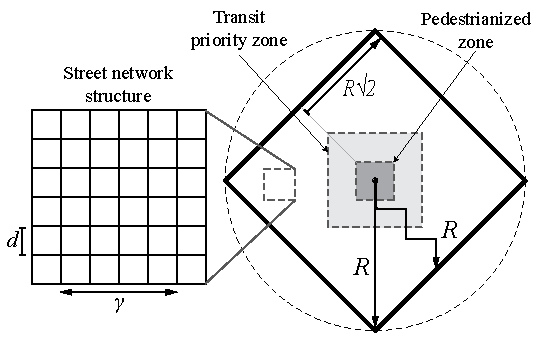
\includegraphics[width=0.5\textwidth]{diagram_pedtransit_grid_city}
     \caption{Rectilinear city with pedestrianized corridor}
     \label{fig:gridcity}
\end{figure}

\noindent The objective is to model the traffic impact on the surrounding street network in order to determine:
\begin{enumerate}[topsep=3pt, itemsep=3pt, partopsep=3pt, parsep=3pt]
    \itshape
    \item what are the optimal pedestrian and transit zone sizes?
    \item what are the impacts on travel time?
    \item what are the resulting shifts in demand?
\end{enumerate}

\section{Demand}
Demand is generated in the city area in units of $\frac{trips}{dist^2}$, and can be simplified into two types: 

\begin{itemize}[topsep=3pt, itemsep=3pt, partopsep=3pt, parsep=3pt]
    \item Uniform baseline travel across the network, $\lambda_b$, and
    \item Monocentric travel demand going to and from the center of the city, $\lambda_c$
\end{itemize}

\noindent The flow across the network at a point $r$ distance from the city center is then the summation of this baseline demand and the monocentric demand, calculated as:

\begin{equation}
    q(r) = \frac{\lambda_b l}{\delta} + \frac{\lambda_c}{4r\delta} \left( \frac{R^2}{r} - r \right)
\end{equation}

\noindent where $l$ is the average trip link length, $\delta$ is the street density in $\frac{lane \cdot dist}{dist^2}$, calculated as $\delta = \frac{4d}{d^2} = \frac{4}{d}$.


\begin{figure}[!ht]
     \centering
     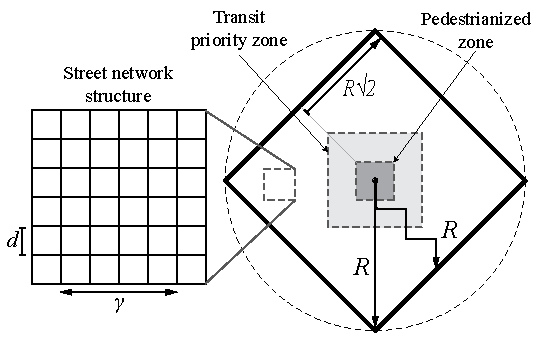
\includegraphics[width=0.5\textwidth]{diagram_pedtransit_grid_city}
     \caption{Diverted route types}
     \label{fig:diverted}
\end{figure}


This function possess the form shown in Figure~\ref{fig:flowacross}. 

Traffic flow on the perimeter road caused by trips being diverted around the zone.



\begin{subequations}
%\footnotesize
\medmuskip=-1mu
\thinmuskip=-1mu
\thickmuskip=-1mu
%\nulldelimiterspace=-1pt
\scriptspace=0pt
\begin{align}
	q_1(\gamma) &= 0 \\
	q_2(\gamma) &= \left[2 \lambda_b \left(R^2 - \gamma^2\right) \times \frac{\gamma^2}{R^2} \times\frac{\gamma}{2}\right] \frac{4s}{8\gamma (R-2)}\\
	q_3(\gamma) &= \left[2 \lambda_b \left(R^2 - \gamma^2\right) \times \frac{\gamma (2R - 3\gamma)}{2R^2} \times  3\gamma\right] \frac{4s}{8\gamma (R-2)}\\
	q_4(\gamma) &= \left[2 \lambda_b \left(R^2 - \gamma^2\right) \times \frac{\gamma (\sqrt{2}R-\gamma)}{R^2} \times  3\gamma\right] \frac{4s}{8\gamma (R-2)}
\end{align}
\end{subequations}





\begin{figure}[!ht]
     \centering
     \hfill
     \begin{subfigure}[b]{0.45\textwidth}
         \centering
         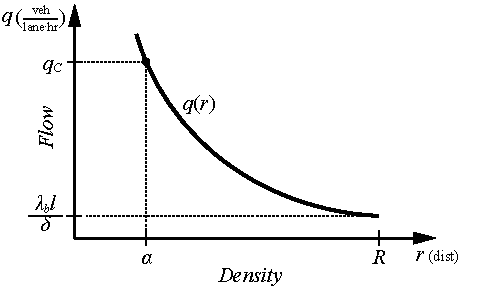
\includegraphics[width=\textwidth]{writing/concept/figures/diagram_flow_across}
         \caption{Trip demand flow at point $r$ distance from center}
         \label{fig:flowacross}
     \end{subfigure}
     \hfill
     \begin{subfigure}[b]{0.45\textwidth}
         \centering
         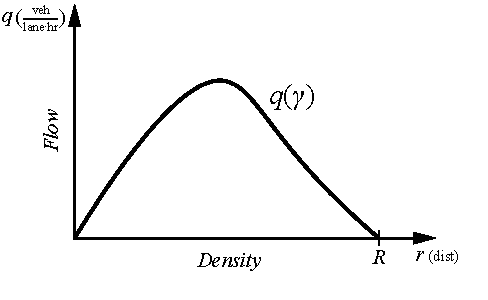
\includegraphics[width=\textwidth]{writing/concept/figures/diagram_perim_flow}
         \caption{Trip demand flow on perimeter of pedestrian zone}
         \label{fig:perimflow}
     \end{subfigure}
     \hfill
     \caption{Macroscopic fundamental diagram and travel time cost function}
\end{figure}

\section{Traffic flow}
Traffic flow through the network is characterized by the macroscopic fundamental diagram (see Figure~\ref{fig:mfd}) as a function of density. A travel time function (see Figure~\ref{fig:traveltime}) then depends upon the state of traffic flow through the network as being either ``uncongested'' (solid line) or ``congested'' (dashed line) in Figures~\ref{fig:mfd} and~\ref{fig:traveltime}.

\begin{figure}[!ht]
     \centering
     \hfill
     \begin{subfigure}[b]{0.4\textwidth}
         \centering
         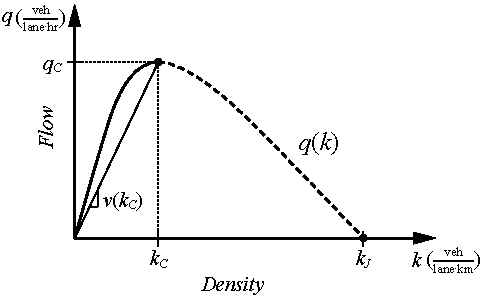
\includegraphics[width=\textwidth]{diagram_mfd}
         \caption{Macroscopic fundamental diagram}
         \label{fig:mfd}
     \end{subfigure}
     \hfill
     \begin{subfigure}[b]{0.4\textwidth}
         \centering
         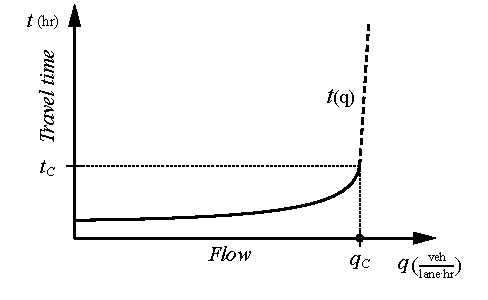
\includegraphics[width=\textwidth]{diagram_traveltime}
        \caption{Macroscopic fundamental diagram}
         \label{fig:traveltime}
     \end{subfigure}
     \hfill
     \caption{Macroscopic fundamental diagram and travel time cost function}
\end{figure}

A travel time cost function can be defined as
\begin{align}
    t(q) &= l \frac{k(q)}{q} & \text{for}~q < \mu \\
    t(q) &= t_c \left(\frac{q}{\mu}\right)  & \text{for}~q \geq \mu
\end{align}

\noindent where $t(q)$ is travel time for flow $q$, $k(q)$ is traffic density for flow $q$, $l$ is link length, and $\mu$ is link capacity. Assuming for this case a parabolic function for the uncongested portion of the flow-density relationship, an expression can be written as

\begin{equation}
    q(k) = q_c - (\alpha k - k_c)^2
\end{equation}

\noindent where $k_c$ is the density at capacity, $q_c$ is the flow at capacity, and $\alpha$ is a fitting parameter. In order to determine travel time using density as a function of flow, $k(q)$, it can be solved for using the quadratic formula

\begin{equation}
    k(q) = \frac{k_c - \sqrt{q_c - q^*}}{\alpha}
\end{equation}

\noindent where $q^*$ is the calculated peak flow required along the parallel streets.


\section{Transit}

Transit travel time is conditional upon whether it operates in a transit priority zone (e.g., dedicated lane or right-of-way) or in mixed-traffic (e.g., city bus). In assuming no other source of delay in a transit priority zone, the travel time of transit is then

\begin{align}
    t_T & = \frac{l}{v_T} + \frac{l}{s}t_s  & \text{with transit priority} \\
    t_T(q) & = l\frac{k(q)}{q} + \frac{l}{s}t_s  & \text{without transit priority when}~q \geq \mu\\
    t_T(q) & = t_c \left(\frac{q}{\mu}\right) + \frac{l}{s}t_s & \text{without transit priority when}~q \geq \mu
\end{align}

\noindent where $V_T$ is the top cruising speed of transit, $s$ is stop spacing, and $t_s$ is stop time. The stop time is essentially the lost time inclusive of acceleration, deceleration and dwell time.






\end{document}
